\documentclass[../../Hardware_Guide]{subfiles}
% Hier müssen keine Packages geladen werden, es werden automatisch die von masterdoc geladen,
% sowie die Konfigurationen.
% Bei includegraphics nur Bildname (Bsp: Bild.png) eingeben, da er in den angegebenen Pfade die Bilder sucht
\graphicspath{{img/}{../../img/}}

\begin{document}

\chapter{Circuit boards}\label{platines}
Beside the ``cardboard'', you will need a camera and a circuit board with infrared LEDs to light the eyes for the camera image. If you want to do binocular eye tracking, you will need two cameras and circuit boards. The circuit board can be etched or can be produced by a perforated grid board. The following components are required for this:
\begin{itemize}
	\item grid board or etched board
	\item 6 IR-LEDs with a beam angle of 20 degrees and a wavelength of 850nm
	\item 13 ohm resistance
	\item micro USB-connector
	\item external power source by micro USB cable (approx. 30cm)
\end{itemize}
Note that the design of the etched board is made for a board-camera like the \textit{ELP 960P HD 1.3 MP}. The hole in the middle fits the width of the camera's objective.\\
The USB port provides 5V power and 500mA current. It's recommended to fix the MicroUSB Port on the circuit board additionally with hot glue. The circuit is a parallel circuit with three branches. Please refer to the circuit board schematic seen on figure \ref{fig:circuit01} or the files for the EDA-program Eagle available on our \href{http://www.bullseye.uol.de}{website}. You can see the circuit boards without components on figure \ref{fig:circuit02} and on figure \ref{fig:circuit03} you can see the circuit boards with components.
\begin{figure}[h]
	\centering
	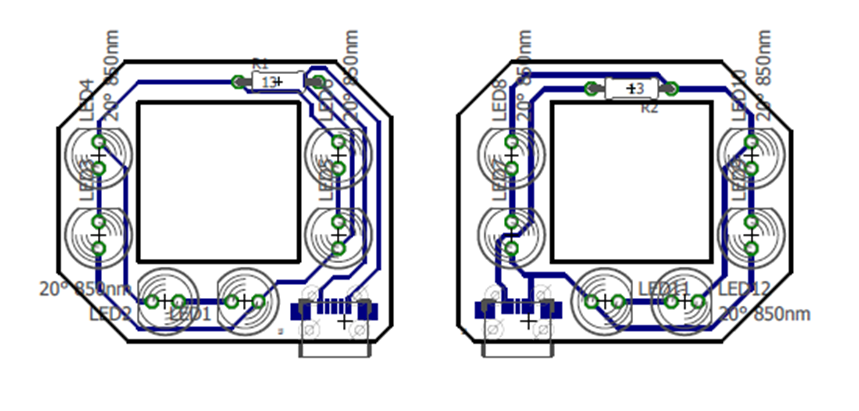
\includegraphics[width=0.7\linewidth]{1}
	\caption{Schematic of the circuit boards}
	\label{fig:circuit01}
\end{figure}
\begin{figure}[h]
	\centering
	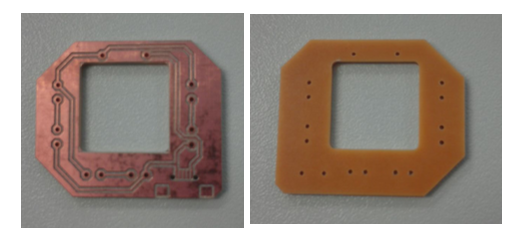
\includegraphics[width=0.7\linewidth]{2}
	\caption{Left: bottom of the etched board, right: top of the etched board}
	\label{fig:circuit02}
\end{figure}
\begin{figure}[h]
	\centering
	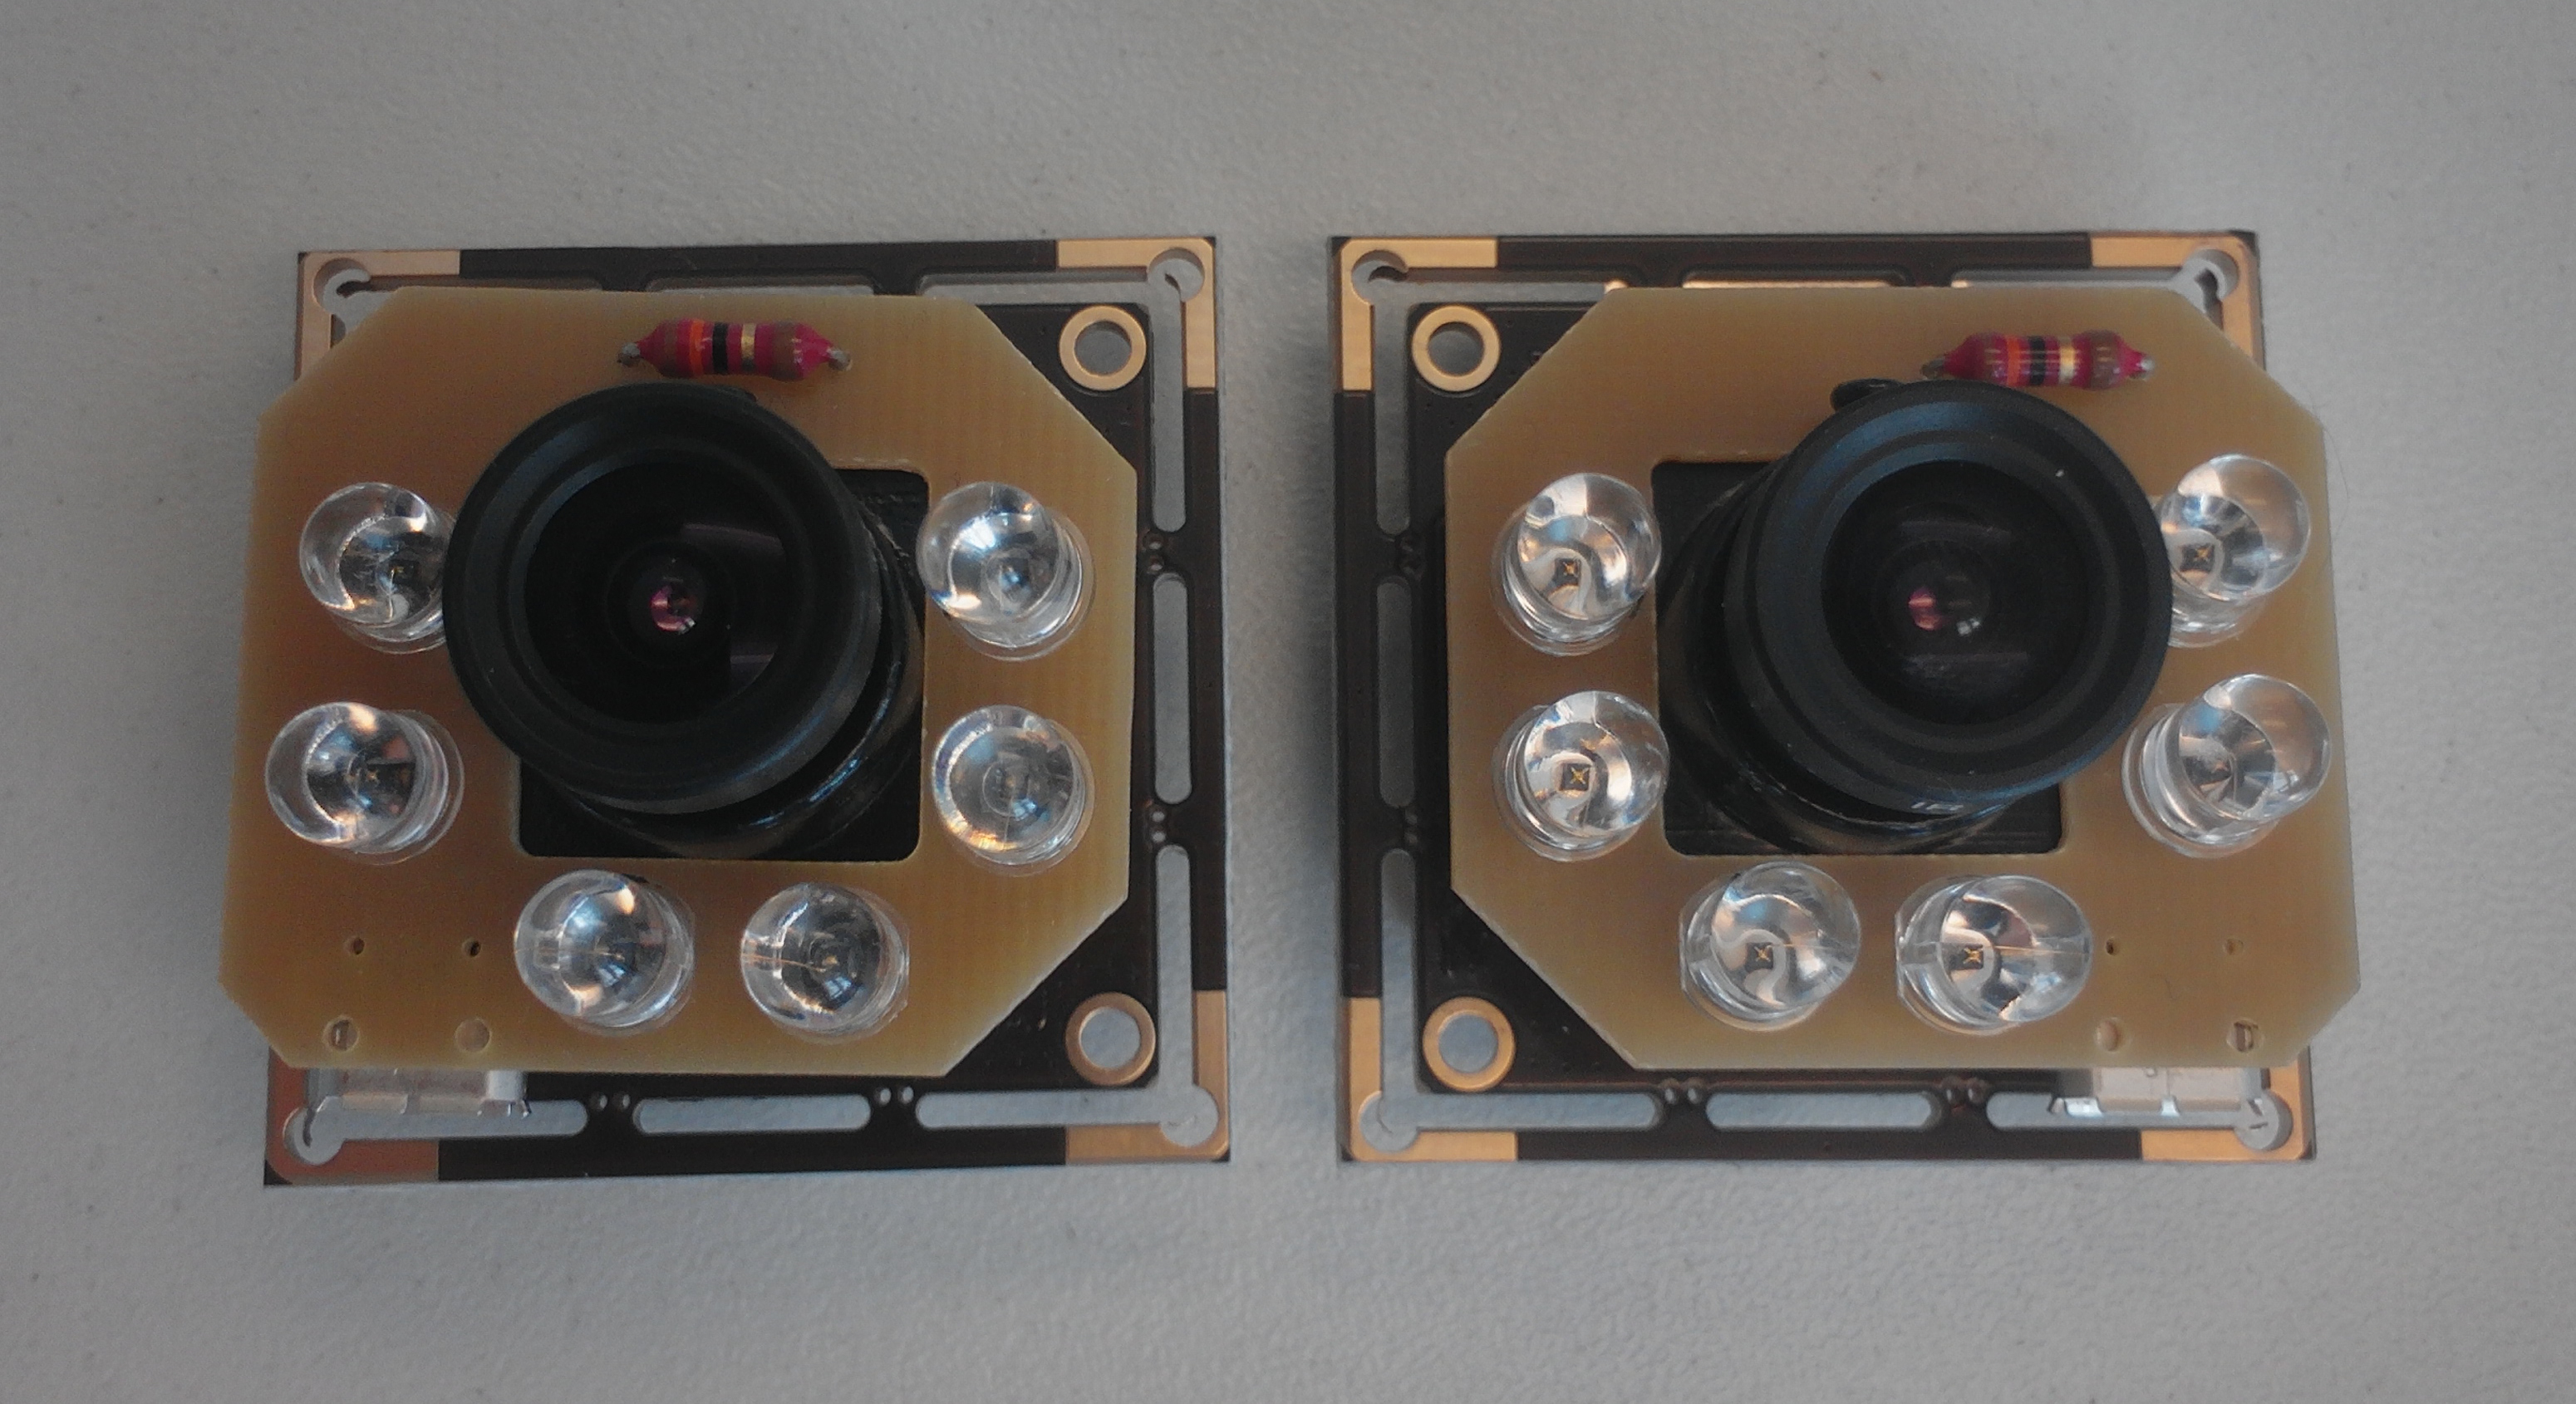
\includegraphics[width=0.7\linewidth]{fertige_Platinen}
	\caption{Equipped circuit boards on the USB cameras}
	\label{fig:circuit03}
\end{figure}
\end{document}